\documentclass{article}
\usepackage[utf8]{inputenc}
\usepackage{amsmath}
\usepackage{listings}
\usepackage{xcolor}
\usepackage{geometry}
\usepackage{graphicx}
\usepackage{subfig}
\usepackage{gensymb}
\usepackage{cancel}
\usepackage{physics}
\usepackage[colorlinks=true]{hyperref}
\definecolor{codegreen}{rgb}{0,0.6,0}
\definecolor{codegray}{rgb}{0.5,0.5,0.5}
\definecolor{codepurple}{rgb}{0.58,0,0.82}
\definecolor{backcolour}{rgb}{0.95,0.95,0.92}
\lstdefinestyle{mystyle}{
    backgroundcolor=\color{backcolour},   
    commentstyle=\color{codegreen},
    keywordstyle=\color{magenta},
    numberstyle=\tiny\color{codegray},
    stringstyle=\color{codepurple},
    basicstyle=\ttfamily\footnotesize,
    breakatwhitespace=false,         
    breaklines=true,                 
    captionpos=b,                    
    keepspaces=true,                 
    numbers=left,                    
    numbersep=5pt,                  
    showspaces=false,                
    showstringspaces=false,
    showtabs=false,                  
    tabsize=2
}

\lstset{style=mystyle}


\title{%
Project 2 - Classification and Regression\\
\Large An exploration of different methods in Machine Learning \\
\large FYS-STK3155 at University of Oslo}
\author{Simen Løken}
\date{November 2020}
\footskip = 110pt
\topmargin = -40pt

\begin{document}
\nocite{articleMedium}
\nocite{mnist}
\nocite{proj2}
\maketitle
\section{Abstract}
In this report, we'll create and maintain multiple different algorithms and methods for solving both classification problems and regression problems. We'll discuss these methods at length, their pros and cons, and weigh them against each other and the data we're working with. We find that for small data sets or when you don't lose to much accuracy in your results, it is preferable to work with smaller algorithms, like logical regression in regards to classification, or just plain stochastic gradient descent for regression when our data sets are sufficiently small.
\section{Introduction}
Imagine if you will that you it's pitch dark outside and you find yourself on a mountain. You've got no vision to guide you, and you wish to make it back down. How would you do it?\newline
It's likely that you answered the rhetorical question above with going downhill. It's the logical thing to do if you want to get down and we can represent a problem like this in mathematics quite simply actually. If we instead imagine our mountain to be a some arbitrary function like this:
\begin{figure}[ht!]
    \centering
    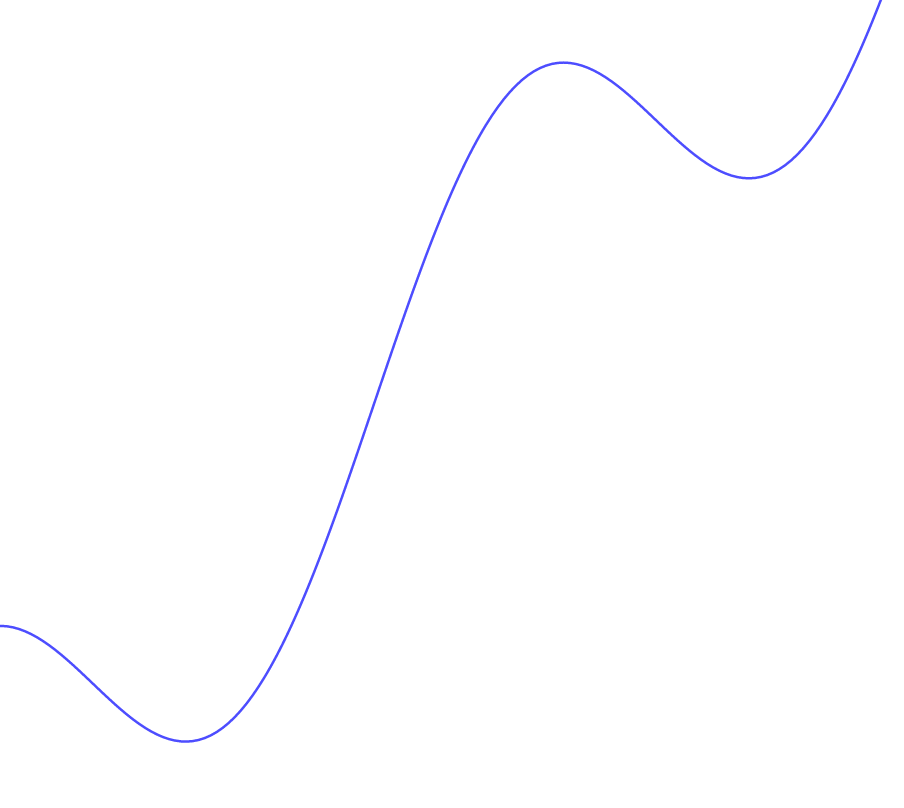
\includegraphics[scale=0.25]{intro1.png}
    \caption{Some arbitrary function with two minimums}
    \label{fig1}
\end{figure}
\newline
The logical approach to finding the bottom in such a scenario would be to use the derivative:
\begin{equation*}
    f'(x) = \frac{\delta f}{\delta x}
\end{equation*}
\newline
which in turn gives us the slope for a given $x$.
\newline
But what if we're working in a three-dimensional space? How would we then go about finding the slope for a given $x$ and $y$.
\newline If you've ever touched calculus, you might recall a handy thing called the gradient:
\begin{equation*}
    \nabla f(x,y) = \left(\pdv{f}{x}\hat{i},\pdv{f}{y}\hat{j}\right)
\end{equation*}
which also happens to return the slope for a given $x$ and $y$ position.
\newline
This is absolutely central to the methods we're going to be discussing here. \newline
Imagine instead that our mountain is a cost function. For most cost functions, the goal is of course to get the lowest value possible, that is, the least error and compromises in our model. So what if we could make a algorithm that uses the gradient in it's current position to approach a local minimum on the cost function, and then retain the values that gave us that answer. \newline
In this report, we're going to be examining problems like these, mainly two different types of problems, regression problems and classification problems, and try different methods on them to see their strengths and weaknesses, before finally doing a critical evaluation of what we've shown and learned. \newpage
\section{Theory and Method}
As we hinted at in the introduction, the bulk of this report is going to be using the method called Gradient Descent (and it's derivatives), so let's take a closer look at these methods:
\subsection{Gradient Descent}
The \textbf{Gradient Descent} method is, in it's most general form, a first order iterative optimization algorithm, which we can use to find a local minimum of a function. \newline
A good illustration of Gradient Descent in action can be seen here:
\begin{figure}[ht!]
    \centering
    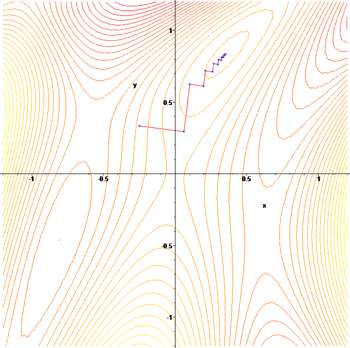
\includegraphics[scale=0.6]{contourWiki.png}
    \caption{A contour-plot showing the movement given by a Gradient Descent method. \newline
    Notice how the function always moves directly "down-stream" from it's position on the surface of the plot. This gives the very characteristic zig-zag of a Gradient Descent method. Note also that it is not a given that we end up at a global minimum \newline
    Image Source: \cite{contourWiki} }
    \label{fig2}
\end{figure} 
This is ideally what we'd wish to accomplish with a Gradient Descent method, but instead of moving toward a function minimum, we're instead moving towards the values that give the lowest error, or rather, the least cost.
\newline
So what does it look like? Mathematically, that is. Well, in it's most general form, imagine that we have some parameter $\theta$ that we wish to minimize. Given what we've already discussed, this $\theta$ could be expressed as:
\begin{equation} \label{1}
    \theta_{i+1} = \theta_i - \eta \nabla f(\theta_i)
\end{equation}
where $\eta$ is the learning rate (timestep) and $\nabla f(\theta_i)$ is the gradient in for the previous parameter $\theta_i$. Notice how the second term is negative, as we're trying to reach minimize our parameter. Conversely, had we instead used Gradient Ascent, the second term would be positive, and we would've instead been looking for a local maximum. \newline
There are however, other versions of the Gradient Descent method, the \textbf{Stochastic Gradient Descent} method is perhaps more popular, as it better serves to minimize bias and potentially find even better values.
\newline Stochastic, from the Greek word 'stókhos', which is a combination of the words 'aim' and 'guess', is essentially interchangeable with the word random in mathematics. As the name suggests, we instead of going through one point at a time, choose a random piece of data to fit to our model. The main purpose this is to speed up workloads of big data sets. In the case of Gradient Descent, we have to run through all of our samples in our training data to update our parameters once, while in the case of Stochastic Gradient Descent, we only run through one data point. \newline
There is however an expansion to the Stochastic Gradient Descent, the \textbf{Stochastic Gradient Descent w/ Mini-batches}. \newline
Here, we instead of choosing only one random point of data, look at a randomly (preferably shuffled as to avoid bias) subset of data. This in turn allows us even faster run times, and allows us to more quickly perform a decent enough fit where our cost function hits a local minimum. \newline
Note that the Equation given in [\ref{1}] does not change between all these three methods. It is only the data we're examining that changes. There are however some modifications that can be done. \newline
The most common way to modify this algorithm would be to include a momentum, which in turn helps slow run times for when our gradient term gets small. This would be:
\begin{equation*}
    v_i = \gamma v_{i-1} + \eta \nabla f(\theta_i)
\end{equation*}
where $v$ is the momentum, and $\gamma$ a momentum parameter. We then get:
\begin{equation}
    \theta_{i+1} = \theta_i - v_i
\end{equation}
Alternatively, an even better method would be to use the Nesterov Momentum, which is given on the form:
\begin{equation*}
    v_i = \gamma v_{i-1} + \eta \nabla f(\theta_i + \eta v_{i-1})
\end{equation*}
giving
\begin{equation}
    \theta_{i+1} = \theta_i - v_i
\end{equation}
Notice that we are essentially time stepping our gradient term using the previous momentum, which in turn converges even faster, saving precious computing time. \newpage
\subsection{Adaptive Methods}
In addition, there are alternative methods that I have dubbed adaptive methods, namely \textbf{Adam} and \textbf{Nadam}. Let's take a look at these:
\newline \textbf{Adam} is an adaptive learning rate optimization algorithm. It updates its weights as follows:
\begin{equation}
    w_t = w_{t-1} - \eta \frac{\hat{m_t}}{\sqrt{\hat{v}} + \epsilon}
\end{equation}
where:
\begin{equation*}
    \hat{m_t} = \frac{m_t}{1-\beta^t_1}
\end{equation*}
\begin{equation*}
    \hat{v_t} = \frac{v_t}{1-\beta^t_2}
\end{equation*}
\begin{equation*}
    m_t = \beta_1 m_{t_1} + (1+\beta_1)\nabla f(\theta_i)
\end{equation*}
\begin{equation*}
    v_t = \beta_1 m_{t_1} + (1+\beta_2)\nabla f(\theta_i)^2
\end{equation*}
retrieved from \cite{Adam} and where $\epsilon$ is a smoothing parameter, to keep us from dividing by zero and $\beta_1,\beta_2$ are forgetting parameters, typically with with values 0.9 and 0.999 respectively. \newline
We can also combine the Adam algorithm with the Nesterov momentum, giving:
\begin{equation}
    \theta_{t+1} = \theta_t - \frac{\eta}{\sqrt{\hat{v}}+\epsilon} \left(\beta_1 \hat{m_t} + \frac{(1-\beta_t)\nabla f(\theta_i)}{1 - \beta^t_1}\right)
\end{equation}
which is commonly referred to as the \textbf{Nadam} method.
\subsection{What are Neural Networks}
So what are Neural Networks? Essentially, neural networks are a way to do machine learning where the computer performs a task after analyzing training samples. This might sound familiar to a normal regression case, which it can be, but quite commonly for, and uniquely, for neural networks is that these examples have been hand-labeled in advance. There are a given set of nodes, or neurons, on each layer. Any given neuron could be connected to many neurons in the previous layer, and it might feed information itself to many neurons in the next layer.
\newline
In it's simplest form, a one-hidden-layer Neural Network could look like:
\begin{figure}[ht!]
    \centering
    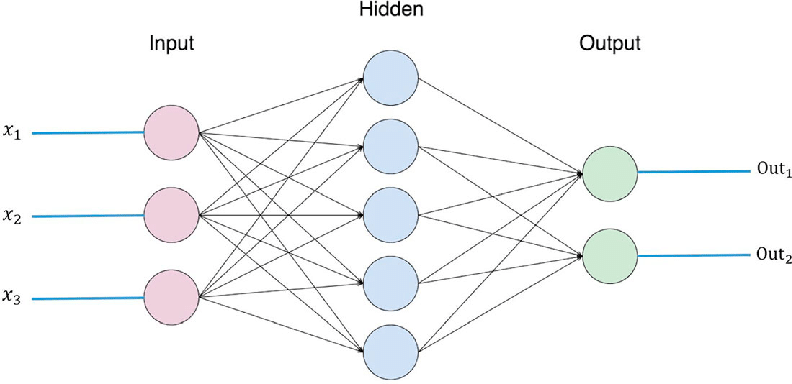
\includegraphics[scale=0.25]{theory1.png}
    \caption{A very simple one-hidden-layer Neural Network with a binary output. \newline
    In our case for the MNIST data, we have 10 outputs, the numbers zero through nine.\newline
    Image Source: \cite{neuralimg1}}
    \label{fig11}
\end{figure}
\newline
For more advanced applications, much more advance than what we're going to examine in this report, you might instead get something like this:
\begin{figure}[ht!]
    \centering
    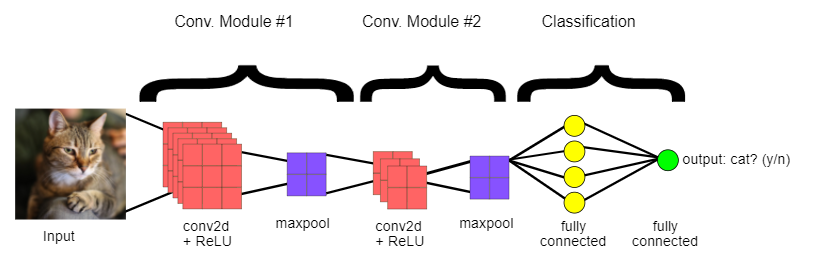
\includegraphics[scale=0.7]{theory2.PNG}
    \caption{A more advanced model using a method of convolutional Neural Networks (abbreviation: CNN) \newline
    Here, data is fed, and then ran through a convolution algorithm and a RELU activation function, before it is subject to max-pooling process. (Max-pooling is reducing the dimensions of the feature map, but still preserving the most important information) \newline
    Image Source: \cite{neuralimg2}}
    \label{fig12}
\end{figure} \newpage
\subsection{Regression vs. Classification}
\textit{So what is the difference between regression and classification?} \newline
They are both methods of machine learning, but let's declare them properly and look at the differences. \newline
\textbf{Regression} is simply put mapping a function, let's say $f$, given from input variables in an array $X$ onto a continuous output variable, $z$. This allows us to look at distribution movement given the data. We've already talked at length about regression in Project 1, so I'll leave it at that for now, but it is an important distinction. \newline
\textbf{Classification} is however, using the same variables, mapping a function $f$, given input variables in an array $X$ onto discrete output variables $z$. That is, we wish to create a model that can read some data, and then try to map it to a set of categories to the best of it's abilities, which means, the main thing separating regression and classification is that when we're working with classification, we're trying to sort the data into an already defined subset, while in regression we're trying to predict some function $f$ given a correlation between data. You cannot for example let a classification problem keep running "beyond" the scope of the data and it should then come as no surprise that we can't solve these two issues in the exact same way.
\subsection{Activation Functions}
We'll also need something called activation functions, which are, in short, functions in a given layer that defines it's output given an input.
\newline
We'll be using mostly ridge activation functions, some of which are:
\begin{equation}
    Sigmoid(x) = \frac{1}{1 + e^{-x}}
\end{equation}
\begin{equation}
    Softmax(x) = \frac{e^{-x}}{\sum e^{-x}}
\end{equation}
\begin{equation}
    Softplus(x) = \ln{\frac{1+e^{k x}}{k}}
\end{equation}

where k is a sharpness parameter. \newline
Additionally, there are the RELU family of activation functions:
\begin{equation}
    RELU(x) = \begin{cases}
                                   0 & \text{if $x<0$} \\
                                   x & \text{if $x\geq0$}
  \end{cases}
\end{equation}
\begin{equation}
    Leaky RELU(x) = \begin{cases}
                                   0.01x & \text{if $x\leq0$} \\
                                   x & \text{if $x>0$}
  \end{cases}
\end{equation}
\begin{equation}
    ELU(x) = \begin{cases}
                                   \alpha(e^{x} - 1) & \text{if $x<0$} \\
                                   x & \text{if $x\geq 0$}
  \end{cases}
\end{equation}
where $\alpha$ is a tweakable parameter. \newline
These were just a few examples, and there are many more activation functions, each with their strengths and weaknesses. \newpage
\subsection{How to evaluate the success of a model}
\textbf{So when all is said and done, how do we know how well we did?} There are different ways to do this. Recall from Project 1 that we discussed the mean squared error:
\begin{equation}
    MSE(y, y_p) =  \frac{\sum_1^{N} (y - y_p)^2}{N} 
\end{equation}
where $y$ is our data and $y_p$ is the predictory data, both of length $N-1$, retrieved after performing the fit. \newline
You may also recall that we discussed $R^2$ score, given as:
\begin{equation}
    R^2(y, y_p) = 1 - \frac{\sum_1^N (y-y_p)^2}{\sum_1^N (y - \Bar{y})^2}
\end{equation}
There are both a great way to properly gauge how well your model has preformed, with the caveat that that model is of a regression problem. However, in this report we're also going to be looking at the very famous MNIST-data, which is entirely a classification problem, so we're going to have to introduce some new methods for gauging. What if we instead decided to compare our real data to the predictory one, and give it one point if it is correct, then divide the total points by the length of the data?
\newline This is called the accuracy, and is a very common tool for gauging the fit of a classification model. In pseudo code, this would be:
\begin{lstlisting}[language=Python]
for i in predictory:
    if i == real_data:
        corr += 1
acc = corr/len(predictory)
\end{lstlisting}
\newline 
Lastly, we also need to define a cost-function for each scenario. \newline
For a regression problem, it is natural to use the mean squared error during the calculation to gauge if we've found a minimum or not, meaning:
\begin{equation}
    C_r(y, P) = MSE(y, P)
\end{equation}
however, it is not so easy for a classification problem. While it is natural for regression to always calculate how far off you were, it is not for classification. \newline
To better illustrate this, say we're working with the MNIST set, and we'd like to sort the numbers. What do we do when the algorithm gets it wrong? Sure, 5 might look like a 6, and it messing up is understandable, but how do we quantify that as an error. \newline
The answer is you can't, or maybe you can, but you shouldn't. Instead, let us use something called the Cross Entropy:
\begin{equation}
    C_c(y, P) = - \sum_{i=1}^N y_i \log{P_i} + (1-y_i) \log{(1-P_i)}
\end{equation}
which, when made as small as possible, should give us the best possible results.
\section{Results}
We first compare a simple Stochastic Gradient Descent with mini-batches to previous methods we have developed in Project 1.
\begin{figure}[ht!]
    \centering
    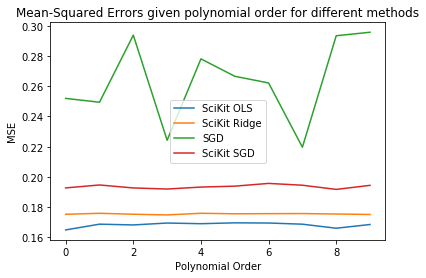
\includegraphics[scale=0.45]{SGDvsOLSvsRidge.png}
    \caption{A plot showing the MSE of own SGD, SciKit's SGD, SciKit's OLS and SciKit's Ridge method for varying polynomial orders.}
    \label{fig3}
\end{figure}
\newpage
Let us now isolate our model, and see how it changes for different variables:
\begin{figure}[ht!]
\centering
\subfloat[Varying learning rate]{
  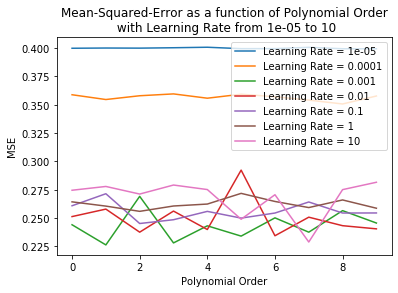
\includegraphics[width=65mm]{SGDLearn.png} \label{a}
}
\subfloat[Varying epoch count]{
  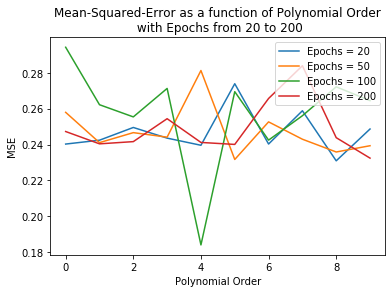
\includegraphics[width=65mm]{SGDEpoch.png} \label{b}
}
\newline
\subfloat[Varying iteration count]{
  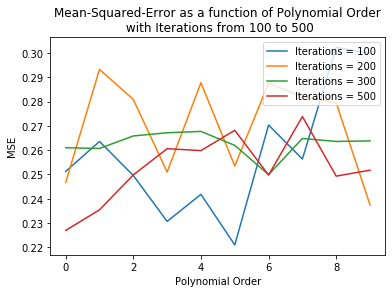
\includegraphics[width=65mm]{SGDIterations.png} \label{c}
}
\subfloat[Varying batch size]{
  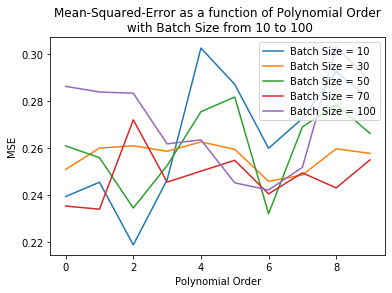
\includegraphics[width=65mm]{SGDBatch.png} \label{d}
}

\caption{Our SGD solution by itself for many different variables.}
\end{figure} \newpage
Let us now examine a FFNN case with regression: \newline
We use our design matrix $X$ and frankedata $z$ from Project 1, and get:
\begin{figure}[ht!]
    \centering
    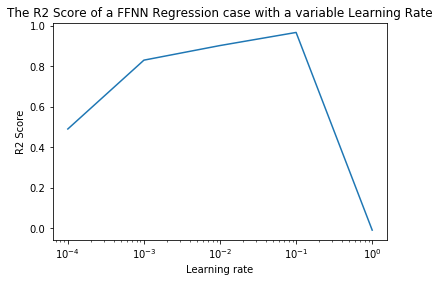
\includegraphics[scale=0.5]{FFNNRegressionR2.png}
    \caption{The R2 Score for a FFNN Regression case with variable learning rate \newline We see clearly that the ideal learning rate for this model is about 0.2, and it gives a very good fit. This is using RELU.}
    \label{fig4}
\end{figure}
\newline
We try again for Sigmoid this time, giving
\begin{figure}[ht!]
    \centering
    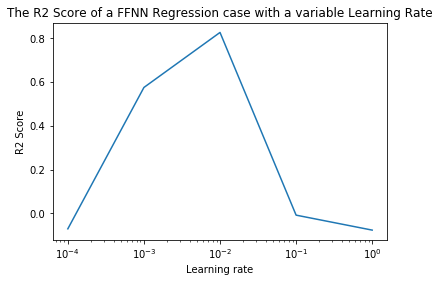
\includegraphics[scale=0.5]{FFNNRegressionR2Sigmoid.png}
    \caption{The R2 Score for a FFNN Regression case with variable learning rate \newline We see clearly that the ideal learning rate for this model is about 0.01, and it gives a very good fit. This is using Sigmoid.}
    \label{fig4}
\end{figure}
\newpage
We now move over to the classification cases. \newline
Let us first examine just the MNIST data alone with variable $\eta$ and $\lambda$, for different numbers of neurons.
\begin{figure}[ht!]
\centering
\subfloat[50 Neurons]{
  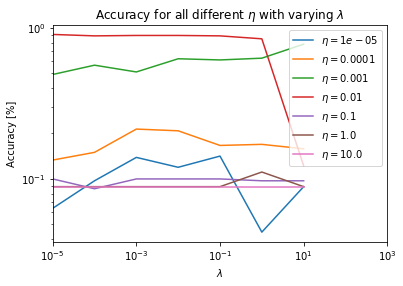
\includegraphics[width=65mm]{MNISTManual50Neuron.png}
}
\subfloat[100 Neurons]{
  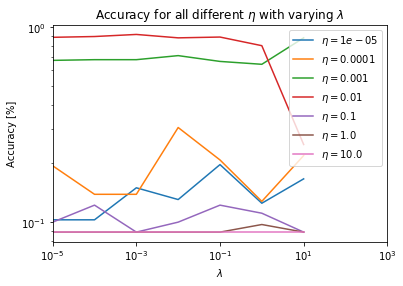
\includegraphics[width=65mm]{MNISTManual100Neuron.png}
}
\caption{Our accuracy for different values of $\lambda$ and $\eta$. First for 50 Neurons and then for 100. Using our own FFNN code.}
\end{figure}
\newline
Let us now look at the Tensorflow version:
\begin{figure}[ht!]
\centering
\subfloat[50 Neurons]{
  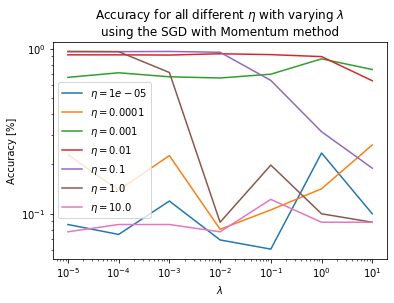
\includegraphics[width=65mm]{MNISTTensor50Neuron.png}
}
\subfloat[100 Neurons]{
  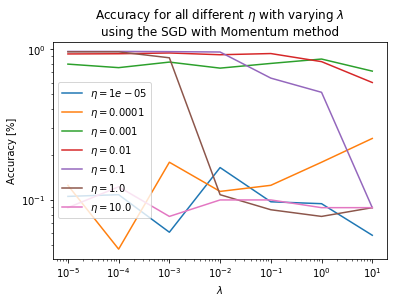
\includegraphics[width=65mm]{MNISTTensor100Neuron.png}
}
\caption{Our accuracy for different values of $\lambda$ and $\eta$. First for 50 Neurons and then for 100. This time using the Tensorflow set of functions.}
\end{figure} \newpage
Finally, let us now examine Logistic Regression.
We use trial and error and find a set of optimal parameters for three methods, GD, SGD and SGD with Mini-batches:
\begin{table}[ht!]
\centering
 \begin{tabular}{||c c c c c c c c c||}
 \hline

 & Iterations & Epoch Count & $\alpha$ & $k$& Batch Size&$\eta$& MSE& R^2 \\ [0.5ex] 
 \hline
 \hline
 GD& 800& 500& 0.6& -& -& 1& 0.019& 0.89  \\
 \hline
 SGD &  600& 200& 0.7& 2.3& -& 0.006& 0.12& 0.32  \\ 
 \hline
 SGD w/ mb &  400& 200& 0.8& -& 50& 0.0005& 0.11& 0.38  \\ 
 \hline
 \hline
\end{tabular}
\caption{A table showing different initial values for Logistic Regression, giving fairly good results. $\alpha$ is a parameter, so is $k$}
\label{tab1}
\end{table}
Let us now examine how Logistic Regression changes for the different variables. For simplicity's sake (and because it's the best model for big data sets, so it's the most relevant), let's use Stochastic Gradient Descent with Mini batches.
\begin{figure}[ht!]
\centering
\subfloat[Varying learning rate]{
  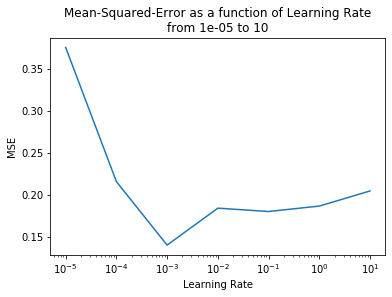
\includegraphics[width=65mm]{LRLearning.png} \label{a}
}
\subfloat[Varying epoch count]{
  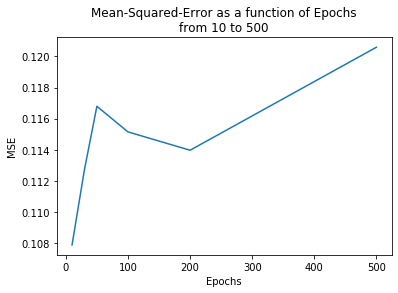
\includegraphics[width=65mm]{LREpochs.png} \label{b}
}
\newline
\subfloat[Varying iteration count]{
  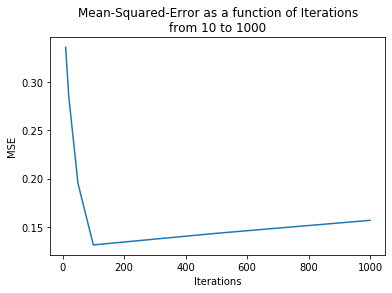
\includegraphics[width=65mm]{LRIterations.png} \label{c}
}
\subfloat[Varying batch size]{
  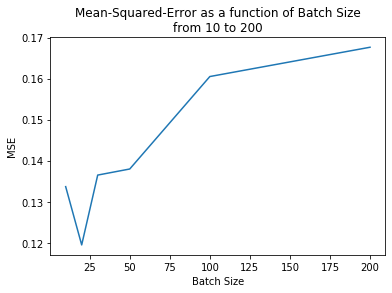
\includegraphics[width=65mm]{LRBatchsize.png} \label{d}
}

\caption{Our Logistic Regression solution for varying values.}
\end{figure}
\section{Discussion}
\subsection*{Run times vs Accuracy for the Gradient Descent Methods}
Looking at our data and what we've seen so far, it may be tempting to call Gradient Descent a surefire winner. With a mean square error as low as 0.02 at its lowest. However, this doesn't show the whole picture. Recall from the theory section where we discussed why we prefer Stochastic over Gradient. \newline
Let's examine these run times. Since I have no proper big data set, let's instead set the polynomial order of our design matrix to be 20, and let it run.
\newline
We get:
\begin{table}[ht!]
\centering
 \begin{tabular}{||c c c c||}
 \hline
 
  &  GD & SGD& SGD w/ mb \\ [0.5ex] 
 \hline
 \hline
 $\eta = 10^-6$& 0.29& 0.41& 0.40   \\
 \hline
 $\eta = 10^-5$&  0.11& 0.40& 0.37  \\ 
 \hline
 $\eta = 10^-4$& 0.044& 0.39& 0.24 \\
 \hline
 $\eta = 10^-3$& 0.023& 0.31& 0.12 \\ 
 \hline
 $\eta = 10^-2$& 0.020& 0.13& 0.17 \\
 \hline
 $\eta = 10^-1$& 0.016& 0.13& 0.18 \\
 \hline
 \hline
 Run time [s]& 474.19& 8.76& 22.34&
 \hline
 \hline
\end{tabular}
\caption{The Mean Square Error for a given learning rate for three Gradient Descent method, and finally the run time.}
\label{tab23}
\end{table}
\newline
It should be obvious to you looking at this table why we shouldn't be using pure Gradient Descent. A design matrix with a polynomial degree of 20 isn't necessarily even that big. It becomes
\begin{equation*}
    X = [N \times 231]
\end{equation*}
where $N$ is the length of the input arrays $x$ and $y$, which also form the corresponding Frankefunction.
\subsection*{Discussing Activation Functions}
Let us discuss a few of the different most popular activation functions, and weigh some of their pros and cons.
\newline The \textbf{Sigmoid} function is perhaps one of the most popular activation functions and for good reason. It's characteristic S-shape means that small changes for $x$ in turn gives large changes in $y$, meaning that $y$ is ideally always large, giving us a distinct advantage when we're looking to classifiy values in a classification case.
\newline In turn though, the S-shape also hurts us when we're far away from $x=0$, because as $x$ increases beyond $\pm 3$ or so, we find an almost flat function, meaning that our gradients become very small, and thus, leaving us "dead in the water" so to speak, if we haven't yet hit our minimum
\newline The \textbf{RELU} function is also a very popular pick, because of it's unique qualities. Studying the RELU function, we see that it returns zero for all negative values of $x$. This in turn means the neuron does not get activated, meaning that only certain neurons are active at a time, and that all active neurons are efficient/actually working/contributing. In turn, this helps computation times for larger data sets. \newline
In turn of course, this also means that we can get permanently inactive neurons, as our gradient for negative $x$ will always be zero.
\newline This is however addressed by the even better \mathbf{Leaky RELU} function, which retains all the previous benefits of the RELU method, but also accounts for the inactive neurons by introducing a new parameter close to zero, so that those neurons can also pass their information forward in the neural network. This makes the Leaky RELU function a good activation function all around.
\newline \textbf{So which one should you choose?} Well, there is no clear cut answer to this. The honest answer is probably that you should try them all and see what gives you the best results, but a general rule of thumb would be that the ones discussed above are usually safe bets.
\subsection*{Discussing Methods - which method is the best?}
So let's get down to the meat of it. Which method is best? The most logical way to tackle this, since we've been looking at two problems for this report, is to look at both regression and classification separately.
\subsubsection*{Classification}
Again, like discussed above. The important thing to look at here would be run times vs. accuracy. Ideally, if a system is solvable within a reasonable margin using logistic regression, then it would follow naturally that that would be best. Neural Networks are computationally expensive, and require both more tweaking (adjusting of parameters) and (in my opinion) work. That being said, if we cannot get sufficiently accurate results with a logical regression, then we need to make use of a neural network.
\newline
Additionally, I'd also like to mention that logical regression is in itself not a classifier, but can be used to make one, where as Neural Networks are.
\subsubsection*{Regression}
For regression however, it is in my opinion not as black and white. We can clearly see in the table above that this too is a case of accuracy vs. run times. \newline
I personally think that the best solution a case of regression would be using the Stochastic Gradient Descent method. My reasoning is that it is both light weight and accurate, like previously mentioned, requires a lot less tinkering for a lot more. While you could of course use a neural network to model a regression case, the benefit is negligible, not to mention Neural Networks are a lot more prone to overfitting, whereas the Stochastic Gradient Descent is a lot more resistant.
\newline
So again, it depends on the complexity of the data set you're analysing, and if you can get away with a simpler method as opposed to a neural network, you should probably do that. \newpage
\subsection*{Confessions}
You might've noticed by now that I have misunderstood part e) entirely. I don't know how it happened, and I didn't notice until friday night (an hour or so prior to the deadline). I was of course supposed to use the Logistic Regression method for classification purposes, not regression purposes
\newline That being said, it should be easy to fix, all that we'd need to do was to instead cast a predictory array $z$ against the true $z$ value, and then binarily decide whether or not they are equal, as discussed in the theory section regarding accuracy. I'd do it if I had the time, and will fix it (after this project is graded). This is part of the reason why I'm a bit past the midnight delivery time, as I have been debating pulling an all-nighter to fix this.
\section{Conclusion}
In conclusion, we've worked with both our design matrix and the MNIST data set so as to visualize and solve both regression and classification problems. We've also looked at and discussed in length the different activation functions, and which ones to use when. \newline
We've lastly shown and discussed some peculiarities with different algorithms, and we've come to the conclusion that for a given problem there is no set in stone answer for what is best, and you should instead choose a solution/solver/method with regards to the material you're working with. That being said, as a general rule of thumb, if you can get away with it, then the lighter computational methods are preferable to neural networks, in terms of computing power vs. result.
\bibliographystyle{plainurl}
\bibliography{citations.bib}
\newpage
\end{document}
